\documentclass{beamer}
\setbeamercovered{dynamic}

\usepackage[ngerman]{babel}
\usepackage{graphicx}
\usepackage[utf8]{inputenc} %deutsche Sonderzeichen
\usepackage{url}

\usepackage[style=apa,sortcites=true,sorting=nyt,backend=biber]{biblatex}
\addbibresource{resources/bib.bib}
\DeclareLanguageMapping{german}{german-apa}

\title{Frankls Kritik des Nihilismus}
\subtitle{Psychologismus und Soziologismus}
\author{Lukas Jox}
\date{16. November 2016}
\institute
{Seminar: Der Wille zum Sinn \\ Humboldstudienzentrum für Philosophie und Geisteswissenschaften}

\usetheme{Warsaw}
\usecolortheme{beaver}

\beamertemplatenavigationsymbolsempty
\setbeamercovered{transparent}

%Trennungsregeln
\hyphenation{Sil-ben-trenn-ung}


\begin{document}

\begin{frame}
\titlepage
\end{frame}

\begin{frame}
\tableofcontents
\end{frame}


%showing page number
\expandafter\def\expandafter\insertshorttitle\expandafter{%
  \insertshorttitle\hfill%
  \insertframenumber$\vert$\inserttotalframenumber}
  
\section{Begriffsklärungen}
\subsection{Wesen des Menschen}

\begin{frame}
\frametitle{Klassischer Dreiklang des Menschen}
\begin{figure}
\centering	
	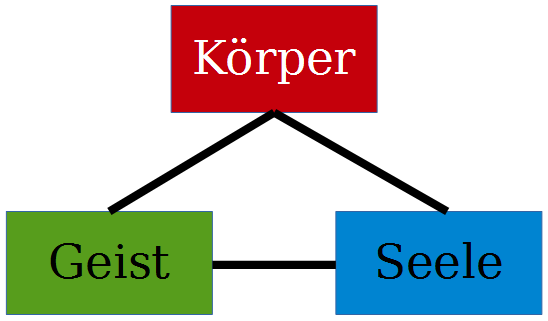
\includegraphics[height=0.5\paperheight]{resources/dreiklang.png}
\end{figure}

\end{frame}


\begin{frame}
\frametitle{Der Dreiklang bei Viktor Frankl (frei nach \textcite{Frankl1996})}
\begin{block}{Seele}
Analog der Psyche Methoden, Operationen, Zustände, Empfindungen
\end{block}
\vspace{0,5cm}
\pause
\begin{block}{Geist}
Sinn, Existenz, Werte, Schöpferisches
\end{block}
\end{frame}


\subsection{Historische Einordnung}


\begin{frame}
\frametitle{Historische Einordnung \parencite{Moog1919}}

\begin{block}{Def. Psychologismus (\citeauthor{Hoefler1906}, \citeyear{Hoefler1906}, S. 322)}
\centering
\textit{\glqq{}ein Zuviel an psychologischem Denken,\\Psychologie am unrechten Ort\grqq{}}
\end{block}

\vspace{0,6cm}

\begin{columns}
   \column[c]{.75\textwidth}
      \begin{itemize}
      \item Beginn mit John Locke (1632--1704) und David Hume (1711--1776), Verbreitung jedoch v.a. im 19. Jahrhunder.
      \item Zu den Kritikern gehörte u.a. Wilhelm Wundt (1832--1920) und Edmund Husserl (1859--1938).
      \end{itemize}
      
%Wobei Wundt zwischen den Fronten steht, da er sich zwar vom Psychologismus abgrenzte, von Husserl jedoch trotzdem dessen bezichtigt wurde      
      
   \column[c]{.25\textwidth}
      %\begin{figure}
         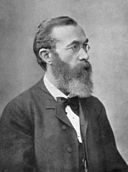
\includegraphics[width=0.7\textwidth]{resources/wundt.jpg}
         \\Wundt (1902)
      %\end{figure}
\end{columns}

\end{frame}


\begin{frame}
\frametitle{Weitere \glqq{}-ismen\grqq{}}

  \begin{block}{Physiologismus/Biologismus}
  	\textit{\glqq{}so läßt er nur Mechanismen und Chemismen gelten; [...] sieht er in einem Lebewesen [...] nur einen Apparat\grqq{}} \footnotesize(\citeauthor{Frankl1996}, \citeyear{Frankl1996}, S.164)\normalsize	
  \end{block}
  
\vspace{0,5cm}
\pause
  
%  $\to$ Historisch eine (Über-)betonung von biologischen Gesetzmäßigkeiten, etwa in verschiedenen Formen des Rassendenkens und im Sozialdarwinismus.

  \begin{block}{Soziologismus}
  	\textit{\glqq{}dass auch für ihn der Mensch zu einem Spielball [...] sozialer Mächte [wird].\grqq{}} \footnotesize(\citeauthor{Frankl1996}, \citeyear{Frankl1996}, S.164)\normalsize
  \end{block}
  
% $\to$ Historisch im Kontext des Marxismus und heute in Bezug auf den Sozialkonstruktivismus verwendet.
  
\end{frame}


\section{Frankl und der Nihilismus}
\subsection{Nihilismus}


\begin{frame}
\frametitle{Frankl und der Nihilismus}

  \begin{block}{}
  	\textit{\glqq{}das Wesen des Nihilismus besteht nicht, wie man anzunehmen pflegt, darin, daß er das Sein verleugnet; er bestreitet [...] den Sinn des Seins.\grqq{}} \footnotesize(\citeauthor{Frankl1996}, \citeyear{Frankl1996}, S.163)\normalsize
  \end{block}
  
\vspace{0,5cm}
\pause
  
  \begin{block}{}
  	\textit{\glqq{}Der Nihilismus demaskiert sich nicht durch das Gerede vom Nichts, sondern maskiert sich durch die Redewendung \textbf{\frqq{}}nichts als\textbf{\flqq{}}.\grqq{}} \footnotesize(\citeauthor{Frankl2015}, \citeyear{Frankl2015}, S.47)\normalsize
  \end{block}
  
\end{frame}


\begin{frame}
\frametitle{aus \textcite{Frankl2015}}

\begin{columns}
   \column[c]{.4\textwidth}
      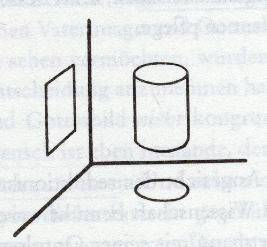
\includegraphics[width=0.7\textwidth]{resources/dimensionen1.png}
      
   \column[c]{.6\textwidth}
      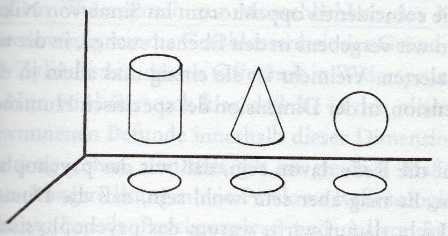
\includegraphics[width=0.75\textwidth]{resources/dimensionen2.png}
\end{columns}

\end{frame}


\subsection{Kritik des Psychologismus}


\begin{frame}
\frametitle{Kritik des Psychologismus}

  \begin{block}{Definition (\citeauthor{Frankl2015}, \citeyear{Frankl2015}, S.43)}
    
    \begin{small}
    {Psychologismus nennt man \glqq{}jenes scheinwissenschaftliche Vorgehen, das aus der seelischen Entstehung eines Aktes auf die Gültigkeit bzw. Ungültigkeit seines geistigen Inhaltes zu schließen Versucht\grqq{}.}    
    \end{small}
    
  \end{block}

  \begin{itemize}
  \setlength{\itemsep}{6pt}
  
    %Schneidergehilfe, kommt "wegen der Ewigkeit", leidet unter der Endlichkeit aller Dinge
  
    \pause
    
    \item geistige Not nicht als psychische Krankheit
    
    \item von der Logik des Menschen zum Existenziellen
    %deshalb immer von Logotherapie und Existenzanalyse her denkend!
    
    \pause
    
    \item[$\Rightarrow$] es gibt neben Soma und Psyche noch etwas drittes (eben das Geistige)
    \begin{itemize}
      \item[$\Rightarrow$] dieses leugnet der Psychologismus
      %Frankl geht es also um einen konkreten Psychologismus, besonders in der therapeutischen Behandlung -> Auseinandersetzung mit der Psychoanalyse
    \end{itemize}
    
    \pause
    
    \item[$\Rightarrow$] Logotherapie als Ergänzung der Psychotherapie
    %"Insuffizienz aller (bisherigen) Psychotherapie", da das Geistige nicht erfasst wird
  \end{itemize}

\end{frame}


\begin{frame}
\frametitle{Kritik des Psychologismus}

  \begin{itemize}
  \setlength{\itemsep}{10pt}
    
    \item \textit{\glqq{}Niemals steht Existenz als Objekt vor mir, vor meinen Augen; sie steht vielmehr immer hinter meinem Denken, hinter mir als Subjekt.\grqq{}} \footnotesize(\citeauthor{Frankl1996}, \citeyear{Frankl1996}, S.170)\normalsize
    \begin{itemize}
      \item[$\Rightarrow$] verwehrt sich der psychischen Analyse
      \item[$\Rightarrow$] der Psychologismus objektiviert diese Geistige Person
    \end{itemize}
    
    \pause    
    
    \item \textit{\glqq{}Geistige Akte sind jedoch ihrem Wesen nach allemal intentional\grqq{}} \footnotesize(\citeauthor{Frankl1996}, \citeyear{Frankl1996}, S.170)\normalsize
    \begin{itemize}
      \item[$\Rightarrow$] in der Intention wieder auf ein Objekt gerichtet
      \item[$\Rightarrow$] durch die Objektivierung der geistigen Akte werden deren eigene Objekte unsichtbar
      \item[$\Rightarrow$] Objekte der Intentionalität sind v.a. (objektive) Werte, der Psychologismus ist also wertblind
    \end{itemize}
    
  \end{itemize}

\end{frame}


\begin{frame}
\frametitle{Psychologismus und Psychoanalyse}

  \begin{itemize}
  \setlength{\itemsep}{10pt}
    
    \item Behebung des Problems einer \glqq{}Psychologie ohne Seele\grqq{} durch Freud
    \begin{itemize}
      \item[$\Rightarrow$] jedoch Verbleiben einer \glqq{}Psychologie ohne Geist\grqq{}, da die Psychoanalyse alles Geistige in die Ebene der Seele projiziert
    \end{itemize}
    
    \pause    
    
    \item Die Reduktion des Menschen auf Triebe ist zu kurz gegriffen
    \begin{itemize}
      \item[$\Rightarrow$] Das Lustprinzip geht von einem \textit{\glqq{}sinnlosen Faktum Lust\grqq{}} aus, es gibt jedoch immer nur \textit{\glqq{}lustvolle Intention\grqq{}}.\\ \footnotesize(\citeauthor{Frankl1996}, \citeyear{Frankl1996}, S.178)\normalsize
      \item[$\Rightarrow$] der Mensch wird nicht \textit{\glqq{}von Triebhaften getrieben, sondern er wird von Werthaftem -- gezogen\grqq{}}. \footnotesize(\citeauthor{Frankl1996}, \citeyear{Frankl1996}, S.179)\normalsize
      %Gleichnis vom Kanalarbeiter, der die Stadt nur als Rohre für Gas und Wasser und Kabel für elektrischen Strom kennt. -> erst durch die Freizeitbegegnung mit Universitäten, Kirchen und Tempeln, Theatern und Museen der Stadt lernt er ihr kulturelles Leben kennen.
    \end{itemize}
  
    \pause  
    %Existenzanalyse als Analyse auf Sinnhaftes im Gegensatz zur Analyse auf Triebhaftes in der Psychoanalyse -> Umkehr der psychoanalytischen Quintessenz   
  
    \item[$\Rightarrow$] \textit{\glqq{}\textbf{\flqq{}}Wo Es ist, soll Ich werden\textbf{\frqq{}}; aber das Ich wird Ich erst am Du\grqq{}}. \footnotesize(\citeauthor{Frankl1996}, \citeyear{Frankl1996}, S.187)\normalsize
  
  \end{itemize}
  
\end{frame}


\subsection{Kritik des Soziologismus}


\begin{frame}
\frametitle{Kritik des Soziologismus}

%Anriss zur Erklärung des Nationalsozialismus, des Zeitgeistes uvm. in seiner anschließenden "Pathologie des Zeitgeistes"

  \begin{itemize}
  \setlength{\itemsep}{10pt}
    \item Reduktion des Menschen auf seine soziale Bedingtheit (und sukzessive vollständige Erklärung aus dieser)

    \pause    
    
    \item Intention einer solchen Erklärungsweise?

    \pause
    
    \item[$\Rightarrow$] Hineinziehen des Objekts in die Bedingtheit des Subjekts
    \begin{itemize}
      \item[$\Rightarrow$] Objekt in Essenz und Existenz abhängig vom Soziologischen
    \end{itemize}
    
    \pause    
    
    \item Der Soziologismus wird damit zum Subjektivismus mit dem Ziel, die Objektivität von Objekten zu tilgen und objektive Werte zu entwerten. \parencite{Frankl1996}
  \end{itemize}

\end{frame}


\begin{frame}
\frametitle{Kritik des Soziologismus}

  \begin{itemize}
  \setlength{\itemsep}{10pt}
  
    \item Der Fehler liegt in einer Verwechslung von Gegenstand und Inhalt
    \begin{itemize}
      \item[$\Rightarrow$] Der Erkenntnis-Inhalt ist \glqq{}bewusstseinsimmanent\grqq{} und daher bedingt.
      \item[$\Rightarrow$] Der Gegenstand der Erkenntnis ist jedoch \glqq{}bewusstseinstranszendent\grqq{} und somit nicht bedingt.
    \end{itemize}  

    \pause  
    
    \item Hierbei geht es eben wieder um \glqq Objekte\grqq  wie Sinn, Gott, Werte.

    \pause  
    
    \item Zentral geht es Frankl auch hier um die Hervorhebung eines Verständnis des eigenständigen geistigen Seins, das durch eine soziologistische wie psychologistische Welterklärung versperrt würde. \parencite{Leser2005}
  \end{itemize}

\end{frame}


\section{Diskussion}


\begin{frame}
  
  \begin{itemize}
  \setlength{\itemsep}{10pt}
  
    \item Stehen wir heute in unserem naturwissenschaftlichen Welt- und Menschenbild (wieder) in der Gefahr eines Psychologismus?
    \begin{itemize}
    
      \pause    
    
      \item[$\Rightarrow$] Etwa im Falle von drängenden Fragen nach Sinn und Existenz? (vgl. den Fall des Schneidergehilfen)
      
      \pause      
      
      \item[$\Rightarrow$] oder auch in unserer psychologischen Klassifikation von Störungen auf der (in Frankls Duktus) seelischen Ebene? (z.B. bei der mit DSM-5 eingeführten Änderung, Trauer im Sterbefall nur zwei Wochen lang als Ausschlusskriterium einer Major Depression zuzulassen)
    \end{itemize}   
  
    \pause  
  
    \item Existieren heutzutage Formen von Soziologismus, etwa in den (extremeren) Theorien der \textit{Gender Studies}?   
  
  \end{itemize}    
  
\end{frame}


\begin{frame}
\printbibliography
\end{frame}

\end{document}